\documentclass[conference]{IEEEtran}
\setlength{\parskip}{0.5em}
\usepackage{graphicx}
\hyphenation{op-tical net-works semi-conduc-tor}

\begin{document}

\title{Challenges of Self-Organisation\\in Agile Projects}


\author{\IEEEauthorblockN{Andrew Hughson}
\IEEEauthorblockA{Dept. of Electrical and Computer Engineering\\
University of Auckland\\
ahug048, 1546814, ahug048@aucklanduni.ac.nz}}


\maketitle


\begin{abstract}

Self-organising teams are one of the twelve key aspects of the Agile
methodology. This essay identifies two concepts which have been identified in
the literature regarding Agile to do with the organisation of self-organising
teams. The first of these is the idea of self-organising teams as a balancing
act regarding their autonomy, cross-fertilisation and self-transcendence. The
second is the roles which have been identified as common in self- organising
Agile teams. The experience of developing an Agile project is relayed in the
context of these concepts and the influence of the roles and tools on the
balances of the self-organising team are analysed.


\end{abstract}


\section{Introduction}

Agile methodologies have seen significant adoption in industry since the release
of the Agile Manifesto \cite{agileadoption} in 2001. One of the key principles
of Agile is self-organising teams. Specifically, the manifesto states that ``The
best architectures, requirements, and designs emerge from self-organising
teams.'' \cite{fowler2001agile}

Self-organising teams are teams which autonomously distribute work among their
members without intervention from upper management. They are composed of
``individuals [that] manage their own workload, shift work among themselves
based on need and best fit, and participate in team decision
making \cite{highsmith2009agile}.''

What is not clear is how self-organising teams organise themselves
\cite{hoda2010organizing}. This essay intends to examine literature on this
topic and relay the experiences gained whilst conducting an Agile project in the
context of a university paper in cooperation with an industry partner.

\section{Related Work}\label{relwork}

Despite the widespread adoption of Agile practices throughout the software
development community, little work has been done in the academic arena with
respect to the Agile feature of self-organising teams \cite{hoda2010balancing}.

\subsection{Balance}

One feature of self-organising teams that has been identified in the literature
is the balancing act that must occur in an Agile organisation. Three specific
conditions of self-organisation were identified by Nonaka et al.
\cite{takeuchi1986new} as being the balance of autonomy, cross-fertilisation,
and self-transcendence.

\begin{figure}[ht!]   \centering
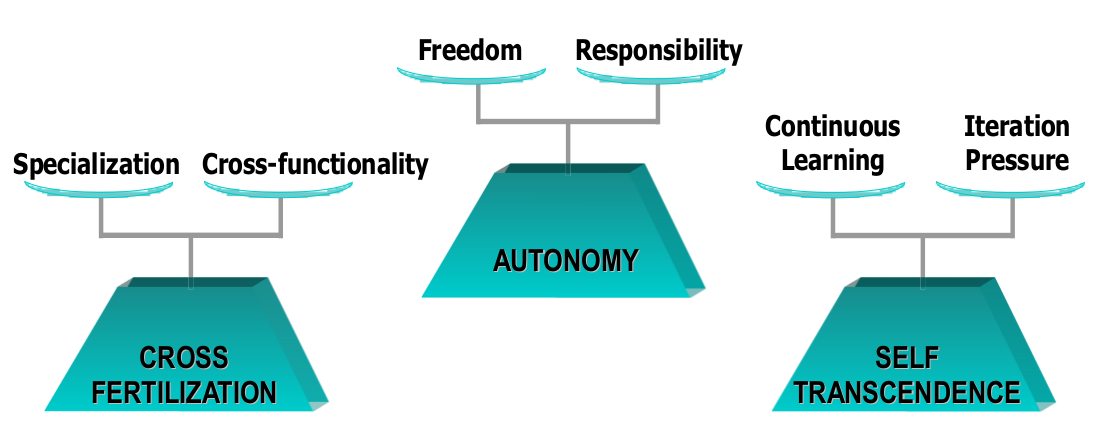
\includegraphics[width=0.5\textwidth]{balancing.png}   \caption{Relationship
between the Balancing Acts and the fundamental conditions of self-organisation
\cite{hoda2010balancing}.} \end{figure}

In a prescriptive software development process senior management is responsible
for setting the goals of the team. Managers assign tasks to specific team
members and perform evaluations of performance and productivity. This stems from
the hierarchical nature of traditional organisations and does not allow
developers to take ownership of the project on which they are working.

In contrast, Agile teams allow members to take ownership of the project on which
they are working by letting them guide development through Agile processes. This
requires Agile teams to be given freedom by upper management to take
responsibility for their project. By giving ownership of the project to the
team, senior management is encouraging members to have a greater sense of
responsibility for the project and hence be more motivated to produce higher
quality work.

With ownership of the project there also comes the freedom to make decisions
about that project, and the responsibility to make good decisions. Agile
facilitates this freedom through certain practices such as sprint planning,
the story board, and sprint retrospectives.

During sprint planning team members have the freedom to decide the direction of
the project for that iteration in terms of what features and work will be done.
The team also has the responsibility to make a plan which is in the best
interests of the project.

Team members also have the freedom to choose their own tasks from the story
board. Here team members have the freedom to practice autonomy by making their
own decisions about which tasks to pick up. The team must also act responsibly
and not choose only easy and low priority tasks from the task board. Fortunately
the transparent nature of the board discourages this through the social pressure
imposed by the need to meaningfully contribute.

The team also has the freedom to reflect and improve on their processes at the
sprint retrospective. Here the team must act responsibly by proactively
identifying their weaknesses and areas of improvement.

If members of a team fail to act responsibly it is the responsibility of senior
management or a terminator \cite{hoda2010organizing} to identify those members
and discipline or remove them from a team. This responsibility also requires
balancing as too much interference from management can jeopardise the ownership
a team feels towards their project \cite{hoda2010balancing}.

An Agile team must also balance its level of cross-fertilisation. According to
Nonaka et al. cross fertilisation requires a team to consist of members of
``varying functional specialisations'' which must interact and work together.
Ideally in an Agile team every member is a master of all trades, though
realistically there is some level of specialisation due to constraints on
resources and time.

The advantages of cross-fertilisation come when members cross-fertilise across
functional roles and cross-technical areas of expertise
\cite{hoda2010balancing}.

By cross-fertilising across functional roles teams can be more adaptive to a
changing workload and can cross barriers between functional specialisations. For
example, having a mix of functional roles can allow developers and testers to
work with one another, whereas when working separately they can often feel as
though they are working against one another.

Cross-fertilising across technical areas of expertise allows for a greater
collective ownership of the project, which is in line with the XP principle of
collective code ownership \cite{beck1999embracing}. If multiple members of a
team are familiar with a technology then it increases the flexibility of the
team and helps members maintain an interest in their work.

Self-transcendence is the principle that teams establish their own goals and
practice continuous evaluation of themselves throughout a project. In Agile this
is achieved through the practices of sprint planning and sprint retrospectives.
Through this practice teams must balance the amount of iteration pressure with
the level of continuous learning \cite{hoda2010balancing}.

Iteration pressure is the pressure induced by time restrictions during a sprint.
While some iteration pressure is desirable as a motivating factor, too much
iteration pressure causes teams to eat into time that could be more productively
spent practising continuous learning. Continuous learning is important for a
team to remain flexible and keep innovating.

\subsection{Roles}

Through a Grounded Theory \cite{strauss1994grounded} study conducted using 24
Agile practitioners in 14 different software organisations in New Zealand and
India, six informal roles were consistently adopted by members of Agile teams
\cite{hoda2010organizing}.

The \emph{mentor} role is played by a member who guides the team through the use
of Agile processes. Despite the simplicity of Agile processes, practising Agile
can be difficult. The Mentor encourages the team to learn and adhere to Agile
practices.

The \emph{co-ordinator} acts as a liaison between the team and the customer. The
co-ordinator gathers initial requirements from the customer and communicates any
changes the customer requires. The co-ordinator is especially important for
teams which are servicing an offshore customer \cite{hoda2010organizing}, as it
is impractical for the entire team to maintain close contact with a customer
which is overseas.

The \emph{translator} translates the requirements gathered by the co-ordinator
from the language of the business domain of the customer into language more
easily understood by the team. They also translate technical language used by
the team into terms more easily understood by the customer. The translator and
the  co-ordinator are often played by the same person in a team.

The \emph{champion} acts as an Agile evangelist to the senior management within
the organisation the team belongs to. Without the support from senior management
Agile teams often fail as they are not allowed the necessary autonomy to
flourish \cite{hoda2010balancing}.

The \emph{promoter} acts as an Agile evangelist to the customers. Agile methods
require a more significant input from the customer than traditional development
methods. This is important as it helps to produce software closer to what the
customer actually wants. The promoter helps the customer to understand Agile
practices and the importance of their involvement in the project.

The \emph{terminator} identifies team members which are having a negative impact
on the productivity of the team. It is sometimes the case that even well
qualified team members do not adapt well to Agile methodologies. It is the
responsibility of the terminator to identify and remove unproductive team
members even without vocalisation of dissent from within the team.

These roles were found to arise organically among the studied teams practising
Agile methodologies. Due to the nature of the study the findings are not
necessarily generalisable to the greater population of Agile teams, yet the
identification of these roles helps provide some insight into the way self-
organising teams organise.

\section{Project Experience}\label{projexp}

The project we undertook from Orion Health is a streamlined check in system
which we dubbed ``Vital Stats Manager'' or ``VSM'' which is intended to replace
paper forms when arriving at a hospital check in. The system consists of four
major components, three of which we tackled over four sprints. These components
are the VSM Android Application, the VSM NFC Receiver, the VSM Server and API,
and the VSM Web Application.

The VSM Android Application \cite{vsmdrd} is intended to be distributed and
installed on patients Android devices. It consists of a form which replaces the
paper form normally filled out when checking in to a hospital. This form allows
patients to enter their vital medical information, such as their height, weight,
allergies, etc.

The VSM NFC Receiver \cite{vsmnfc} is the component of the system which was not
fully developed over the four sprints of the project due to limitations in the
availability of required NFC hardware. For the purposes of the project a mock
receiver was developed as an Android application, though the user interface was
not a focus. The role of this component is to receive patient check ins. At the
reception of each hospital department it is envisioned that there will be one of
these receivers which a patient can touch with their Android device with the VSM
Android Application installed. By touching the receiver they transmit their
vital information to the hospital and are checked in.

The VSM Server and API \cite{vsmsvr} component is the component which receives,
stores, and exposes patient check ins. When a patient checks in by transmitting
their vital information over NFC to the receiver, the receiver uploads the
received data to the server which stores it in a database. This information is
then exposed via a RESTful API for consumption by other components of the
system.

The VSM Web Application \cite{vsmsvr} is the main consumer of the data exposed
by the VSM Server and API. It is intended that receptionists and nurses can see
recent check ins to a department and review and edit patient vital information
as patients check in to the hospital. It provides functions to search, filter,
edit and delete patients.

The team for this project consisted of six members; myself, Michael Little,
Jourdan Harvey, Dave Carpenter, Andrew Luey, and Thomas Lugnet. This team was
self assembled before the project requirements were available. Each member was
familiar with the others and had differing degrees of software development
experience.

% After receiving the project description and before our first meeting with our
% customer representatives we decided to work on a prototype of the system based
% on our understanding of the requirements. This gave the team an opportunity to
% research and familiarise themselves with the technologies which would be used to
% develop the final working system.

% At our first meeting with our customer representatives we clarified the project
% requirements and realised our understanding was not complete. Fortunately our
% prototypes of the system components were modifiable to the point where this was
% not a large concern and our technology choices were not affected. Here we see an
% example of the way Agile teams can react more easily to changes in requirements,
% due to the short iterations and frequent customer interaction our software was
% able to adapt easily.

After gathering the requirements from our first meeting with our customer
representatives we self organised into pairs roughly mapping to the three
components which we were to implement. Particular members of our team had more
experience in different areas of development. This was important with regard to
the manner in which we self organised. Dave and myself had experience in back
end development relevant to the Server and API, Michael had experience in
Android development, and Dave, Jourdan and I had experience in web front end
development.

To encourage our team members to become ``masters of all trades'' and avoid too
much specialisation we organised pairs so that a member with experience in the
area of the system they were developing was paired with a member with less or no
experience in that area. By practising pair programming members were able to
undergo cross-fertilisation, learning about the technologies and the
implementation details of the part of the system on which they were working. In
this manner we avoided any one team member becoming a specialist, though there
was a difficulty in balancing our self-transcendence. This can be attributed to
the time constraints of the project and iteration pressure that this caused.

Three pairs ended up forming - myself and Andrew Luey worked on the VSM Server
and API. I had experience in developing RESTful APIs backed by databases similar
to the way this component was going to work. Michael had previous Android
development experience and so Jourdan and Michael worked on the VSM Android
Application. Dave had some limited experience in web development and so Dave and
Thomas worked on the VSM Web Application.

Despite certain members having relevant experience, the specific technologies we
chose were not necessarily familiar. Those members with experience could more
easily pick up these new technologies and therefore expedite the learning of
those less experienced members. As an example of this cross-fertilisation, we
used an ORM called SQLAlchemy to interface with our database in the VSM Server
component. I was able to quickly pick up this technology from my previous
experience with different ORMs and in the process teach Luey the important
aspects necessary for the development of our system.

Over the development of the project we had roughly weekly meetings with our
customer representatives from Orion Health - that is two meetings per sprint. As
Agile practitioners themselves they took on the mentor role as well as the role
of translator.

In their role as mentors they advocated certain Agile practices to us -
especially test driven development. We managed to incorporate this technique
more and more as our software stabilised and we became more familiar with the
technologies we were using.

As customers our representatives at Orion provided us with the requirements for
the project. As developers themselves they were able to translate the domain
knowledge from the health industry to more consumable information for us as
developers. As the project progressed and we completed the original user stories
and met milestones they would add requirements to the project. Here we see
another example of Agile methodologies and the way requirements can change and
planning can occur at late stages of the project, as opposed to more
prescriptive methodologies in which changes may be more difficult to
incorporate.

Some examples of late requirements added by our customers were the additions of
department log ons and breadcrumbs. The customers asked for the ability to
separate patients by departments and let nurses and administrative staff see
only those patients from specific departments. This requirement was added in the
fourth sprint of the project after we had become familiar with our code and the
technologies we were using. This gave us an opportunity to practice TDD. The
main change had to occur in the server where we needed to change the way
patients were accessed to limit them to departments. We were able to add tests
which would verify the correctness of our implementation and then implement the
changes. From this we saw the value of the red-green-refactor cycle.

The second requirement - the addition of breadcrumbs to the web interface - was
also introduced in the fourth sprint. At this point we were able to become more
cross functional as a team as we had overcome the learning phase. As a result I
was able to work on this requirement which was outside of the VSM Server
component I had been mainly responsible for up to this point. Given more time I
can see how this could have occurred in other places with other members as work
would run out in specific areas and members would be required to undertake tasks
in unfamiliar areas of the code base.

The tool we used throughout development for organising work was GitHub. GitHub
acts as a source control repository and issue tracker. The issue tracker allowed
us to add tasks to certain milestones and assign them to members. It also
allowed us to implement code reviews through a feature called ``pull requests.''

The issue tracker was used as the mechanism for which work was distributed
throughout the team. At the beginning of an iteration after our sprint planning
and retrospective we would create issues which represented the tasks which we
intended to complete in that iteration. These tasks were then available to be
picked up by any member who wished to undertake them. Issues were also logged as
development occurred and new requirements were recognised or bugs found. For
example, while developing the NFC Receiver which would upload patient
information to the server, Michael and Jourdan would identify bugs and issues
they had with the RESTful API. By logging these on GitHub everyone would receive
an email with the bug report, allowing anyone to pick up and comment on the bug.

The GitHub issue tracker was the key to our team's balance of autonomy and
responsibility. GitHub also has a feature that tracks the number of lines and
commits to a repository by a user. These two features combined provided the
mechanism and the motivation to be responsible while also being autonomous. As
an analogue to the story board it has an advantage because it does not require
the team to be co-located, a great advantage to us due to our scheduling
conflicts.

``Pull requests'' are the key feature of GitHub which democratise code reviews.
Whenever a feature or bug fix was finished on a branch, a member could open a
pull request, requesting their code be integrated into the master branch. All
other members would then receive an email and are able to discuss the changes,
comment on specific lines of code, add their own commits to the changes, and
eventually approve the pull request for merging. This feature was also part of
helping the team to maintain cross-functionality as it made it easy to monitor
the changes to the system as the code developed.


\section{Discussion}

Many of the concepts from section \ref{relwork} came to bear throughout the
experience of developing Vital Stats Manager in co-operation with Orion Health.

\subsection{Balance}

With regards to balancing, we did well when it came to autonomy and cross-
fertilisation, though we did face challenges with self-transcendence.

In the role of senior management, Dr. Rashina Hoda provided our group with the
freedom to practice autonomy. Because of our social connection with one another,
the tools provided to us by GitHub and the mentorship of our customer
representatives we were able to balance this freedom responsibly and do a fair
amount of work evenly distributed among the team during each iteration.

I have described in section \ref{projexp} how through practising pair
programming and through using GitHub's pull request tool we were able to cross-
fertilise across functional roles. Given more time I would have expected this
balance to improve as we managed to cross-fertilise across areas of technical
expertise, allowing members to become more cross-functional.

The main challenge we faced throughout the project was iteration pressure. The
technologies used in this project were largely new to all of us and so required
an investment in time to practice continuous learning. With the limited time
available to work on the project this led to iteration pressures which created a
larger degree of specialisation than would be otherwise optimal. This resulted
in the creation of the three subgroups. As stated earlier this was mitigated in
later iterations as the burden of continuous learning on our time constraints
lessened.

\subsection{Roles}

Not all of the roles which were identified by Hoda et al.
\cite{hoda2010organizing} were evident in our experience of Agile. Particularly,
nobody took on the roles of champion, promoter, or terminator, largely due to
the setting in which the project was undertaken. Agile was a given for this
project and a mechanism was not available to ``terminate'' somebody from the
group.

As stated in section \ref{projexp} our customer representatives undertook the
role of mentors. As Agile practitioners themselves they would ask us about the
aspects of the methodologies that we were using and which we found most useful.
They also reiterated the importance of agile practises, particularly sprint
planning and retrospectives and TDD.

Our customer representatives also undertook the role of translators. As software
developers in the field of health software they were uniquely poised to help
translate the business needs of hospitals into terms which were easy to grasp
for us as software developers. A particular example of this is ``vital
statistics.'' On hearing this term initially we assumed it meant things such as
heart rate, body temperature, etc. This was clarified for us by our translators
as meaning the information you provide when you check in to a hospital.

A not insignificant portion of our communication with our customer
representatives was undertaken via email. To reduce complexity Dave Carpenter
was nominated as customer liaison and undertook the role of co-ordinator. Any
clarifications we required or extra communication went though Dave in this role.
Having this single point of contact smoothed our relations with the customers
and made it easy to know where to go when further information was needed.

\section{Implications for Practice}

The key pieces of knowledge to take from our experiences with Agile in the
context of the concepts outlined in section \ref{relwork} are as follows:

\begin{itemize}

  \item Have senior management which is supportive of Agile and provides the
necessary freedom.

  \item Use tools which support the balances of autonomy and cross-
fertilisation.

\end{itemize}

If senior management is not in support of the project and does not provide the
necessary freedom to the team, it may be a good idea to employ the role of
champion. The balance of autonomy was key to the success of the Vital Stats
Manager project. The ability to self-organise without worrying about pleasing
upper management (the lecturer) contributed greatly to the feeling of ownership
that the team had for the project, greatly improving the amount of effort put in
and the quality of the final product.

GitHub was another key component to the success of the project. Its features
provided a platform on which our team was able to perform the balancing act
required for a successful project. As a tool GitHub allows a team to practice
Agile processes without being strongly process oriented. The issue tracker is a
great aid to a team's autonomy, while the pull request feature keeps everyone in
the loop on new features, which is surprisingly important to the process of
cross-fertilisation.

\section{Conclusion}

As we have seen, the organisation of self-organising teams is a balancing act
across the three features of autonomy, cross-fertilisation and self-
transcendence.

With the support of senior management and the proper employment of Agile roles
a self-organised team can be very productive, given the sense of ownership they
gain via cross-functionality and autonomy.


\section*{Acknowledgement}

I would like to thank the members of Best Group for their contributions to the
Vital Statistics Manager project. I would also like to thank our mentors from
Orion Health for their guidance and advice throughout the project. Finally I
would like to thank Dr. Rashina Hoda and Mr. Howard Wang for running the course
this semester.


\bibliographystyle{IEEEtran}
\bibliography{essay}


\end{document}
